\documentclass[11pt,a4paper]{article}
\usepackage[utf8]{inputenc}
\usepackage{amsmath}
\usepackage{amsfonts}
\usepackage{amssymb}
\usepackage{graphicx}
\usepackage{tikz}
\usepackage[left=2cm,right=2cm,top=2cm,bottom=2cm]{geometry}
\author{Paul LANDRIER}
\title{Provenance sur les réseaux de neurones}
\date{}

\usetikzlibrary{arrows.meta, positioning}


\begin{document}
\maketitle

\section{Exemples}

	\subsection{Réseaux de neurones}

On s'intéresse d'abord à des réseaux de neurones denses avec une fonction d'activation $f$.

\begin{figure}[!h]
\centering
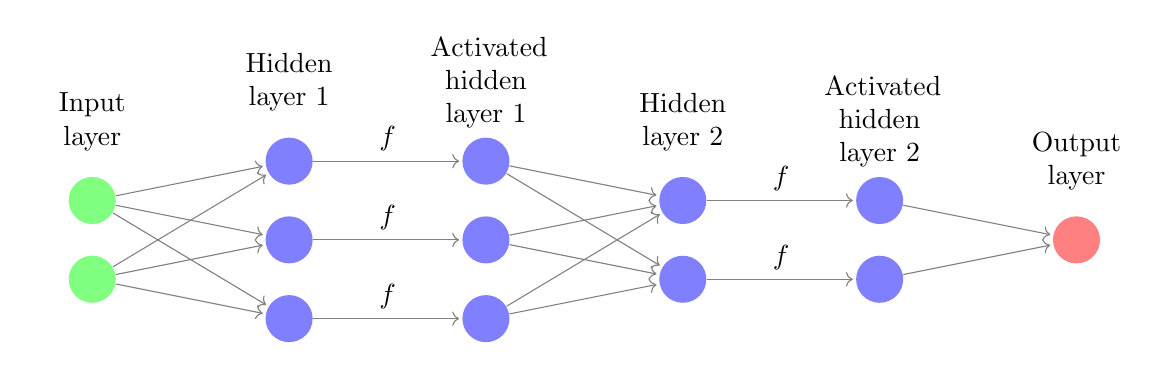
\begin{tikzpicture}[shorten >=1pt,->,draw=black!50, node distance=\layersep]
\tikzstyle{neuron}=[circle,fill=black!25,minimum size=17pt,inner sep=0pt]
\tikzstyle{input neuron}=[neuron, fill=green!50];
\tikzstyle{output neuron}=[neuron, fill=red!50];
\tikzstyle{hidden neuron}=[neuron, fill=blue!50];
\tikzstyle{annot} = [text width=4em, text centered]

% Specify the distance between layers
\def\layersep{2.5cm}

% Draw the input layer nodes
\foreach \name  in {1,2}
  \node[input neuron] (I-\name) at (0,1.5-\name) {};
  
% Draw the hidden layer 1 nodes
\foreach \name in {1,2,3}
  \node[hidden neuron] (H1-\name) at (\layersep, 2 -\name) {};
  
% Draw the activated hidden layer 1 nodes
\foreach \name in {1,2,3}
  \node[hidden neuron] (H1-act-\name) at (2*\layersep, 2 -\name) {};

% Draw the hidden layer 2 nodes
\foreach \name in {1,2}
  \node[hidden neuron] (H2-\name) at (3*\layersep,1.5-\name) {};
  
% Draw the activatec hidden layer 2 nodes
\foreach \name in {1,2}
  \node[hidden neuron] (H2-act-\name) at (4*\layersep,1.5-\name) {};

% Draw the output layer node
\node[output neuron] (O) at (5*\layersep,0) {};

% Connect every node in the input layer with every node in the hidden layer 1
\foreach \source in {1,2}
  \foreach \dest in {1,2,3}
    \path (I-\source) edge (H1-\dest);
    
% Connect every node in the first hidden layer with its activated counterpart
\foreach \node in {1,2,3}
  \path (H1-\node) edge node[midway,above] {$f$} (H1-act-\node);

% Connect every node in activated hidden layer 1 with every node in hidden layer 2
\foreach \source in {1,2,3}
  \foreach \dest in {1,2}
    \path (H1-act-\source) edge (H2-\dest);
    
% Connect every node in the second hidden layer with its activated counterpart
\foreach \node in {1,2}
  \path (H2-\node) edge node[midway,above] {$f$} (H2-act-\node);

% Connect every node in activated  hidden layer 2 with the output layer node
\foreach \source in {1,2}
  \path (H2-act-\source) edge (O);

% Annotate the layers
\node[annot,above of=I-1, node distance=1cm] {Input layer};
\node[annot,above of=H1-1, node distance=1cm] {Hidden layer 1};
\node[annot,above of=H1-act-1, node distance=1cm] {Activated hidden layer 1};
\node[annot,above of=H2-1, node distance=1cm] {Hidden layer 2};
\node[annot,above of=H2-act-1, node distance=1cm] {Activated hidden layer 2};
\node[annot,above of=O, node distance=1cm] {Output layer};

\end{tikzpicture}
\label{fig:nn_ex}
\caption{Réseau de neurone $N$}
\end{figure}

On appelle respectivement $E,H_1,H_1',H_2,H_2'$ et $o$ les vecteurs représentant les couches successives. On définit $(A_1,B_1)$, $(A_2,B_2)$ et $(A_3,B_3)$ les couples matrices vecteurs tels que $H_1=A_1 E + B_1$, $H_2 = A_2 H_1' + B_2$ et $o=A_3 H_2' + B_3$.

 En écrivant explicitement l'exécution générale, on obtient :
 
\newcommand{\h}[2]{a^{#1}_{#2 , 1}x_1 + a^{#1}_{#2 , 2}x_2 +b^{#1}_{#2}}
\newcommand{\hbig}[5]{a^{#1}_{#2 , 1} #3 + a^{#1}_{#2 , 2} #4 + a^{#1}_{#2 , 2} #5 +b^{#1}_{#2}} 
 
\begin{itemize}
 
	\item  $E = \left( \begin{array}{c} x_1 \\ x_2 \end{array} \right)$
 
	\item $H_1 = A_1 E + B_1= \left( \begin{array}{c} \h{1}{1} \\ \h{1}{2} \\ \h{1}{2} \end{array} \right)$
 
	\item $H_1' = f(H_1) = \left( \begin{array}{c} f(\h{1}{1}) \\ f(\h{1}{2}) \\ f(\h{1}{3}) \end{array} \right)$
 
	\item $H_2 = A_2 H_1' +B_2 =$\\
	$\left( \begin{array}{c} 
	\hbig{2}{1}{f(\h{1}{1})}{f(\h{1}{2})}{f(\h{1}{3})} \\
	\hbig{2}{2}{f(\h{1}{1})}{f(\h{1}{2})}{f(\h{1}{3})} 
	\end{array} \right)$
	
	\item $H_2' = f(H_2) = $\\
	$\left( \begin{array}{c} 
	f(\hbig{2}{1}{f(\h{1}{1})}{f(\h{1}{2})}{f(\h{1}{3})}) \\
	f(\hbig{2}{2}{f(\h{1}{1})}{f(\h{1}{2})}{f(\h{1}{3})})
	\end{array} \right)$

	\item 
	$o = a^{3}_{11}f(\hbig{2}{1}{f(\h{1}{1})}{f(\h{1}{2})}{f(\h{1}{3})})$ \\
	$+ a^{3}_{22} f(\hbig{2}{2}{f(\h{1}{1})}{f(\h{1}{2})}{f(\h{1}{3})})$

\end{itemize}

\subsection{Graphes de calculs}

Les graphes de calculs sont une autre façon de représenter l'exécution d'un réseau de neurones, en mettant en évidence la structure des calculs.

Commençons par un exemple. Nous définissons la fonction $f(x,y,z)=xe^{(x^2-y^2)z}$. Son graphe de calcul est représenté en Figure \ref{fig:ex_graphe_calcul}.

\begin{figure}[!h]
\label{fig:ex_graphe_calcul}
\centering

\begin{tikzpicture}[node distance=15cm]

    % Nodes
    \node[draw, rectangle] (x) at (0, 0) {$x$};
    \node[draw, rectangle] (y) at (0, -2) {$y$};
    \node[draw, rectangle] (z) at (6, -3.5) {$z$};

    \node[draw, circle] (a) at (3, 0) {$a=x^2$};
    \node[draw, circle] (y2) at (3, -2) {$b=y^2$};
    \node[draw, circle] (x2miny2) at (6, -1) {$c=a - b$};
    \node (minsymb) [left=0.15 of x2miny2] {$-$};
    \node[draw, circle] (prod) at (9, -2) {$d=cz$};
    \node (multsymb) [left=0.15 of prod] {$\times$};
    \node[draw, circle] (exp) at (12, -2) {$e=e^d$};
    \node[draw,circle] (prodfin) at (15,-1) {$g=xe$};
    \node [left=0.15 of prodfin] {$\times$};
    \node (out) at (17.5,-1) {$f(x,y,z)$};
    
    % Arrows
    \draw[->] (x) -- node[midway,above] {$t \mapsto t^2$} (a);
    \draw[->] (y) -- node[midway,above] {$t \mapsto t^2$} (y2);
    \draw[->] (a) -- (x2miny2);
    \draw[->] (y2) -- (x2miny2);
    \draw[->] (x2miny2) -- (prod);
    \draw[->] (z) -- (prod);
    \draw[->] (prod) -- node[midway,above] {$t \mapsto e^t$} (exp);
    \draw[->] (exp) -- (prodfin);
    \path[bend left=30] (x) edge (prodfin);
    \draw[->] (prodfin) -- (out);

\end{tikzpicture}
\caption{Graphe de calcul de la fonction $f$}
\end{figure}

Pour le réseau de neurones $N$, en considérant les opérations sur les vecteurs, cela donne :

\begin{figure}[!h]

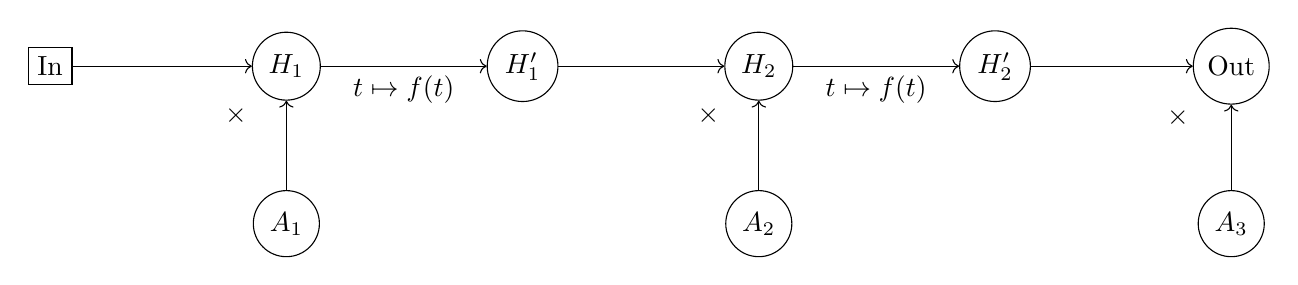
\begin{tikzpicture}

\node[draw,rectangle] (Inputs) at (0,0) {In};
\node[draw,circle] (H1) at (3,0) {$H_1$};
\node[draw,circle] (H1') at (6,0) {$H_1'$};
\node[draw,circle] (H2) at (9,0) {$H_2$};
\node[draw,circle] (H2') at (12,0) {$H_2'$};
\node[draw,circle] (Output) at (15,0) {Out};

\node[draw,circle] (A1) at (3,-2) {$A_1$};
\node[draw,circle] (A2) at (9,-2) {$A_2$};
\node[draw,circle] (A3) at (15,-2) {$A_3$};

\draw[->] (Inputs) -- (H1);
\draw[->] (H1) -- node[midway,below] {$t \mapsto f(t)$} (H1');
\draw[->] (H1') -- (H2);
\draw[->] (H2) -- node[midway,below] {$t \mapsto f(t)$} (H2');
\draw[->] (H2') -- (Output);

\draw[->] (A1) -- (H1);
\draw[->] (A2) -- (H2);
\draw[->] (A3) -- (Output);

    \node [below left=0.1 of H1] {$\times$};
    \node [below left=0.1 of H2] {$\times$};
    \node [below left=0.1 of Output] {$\times$};


\end{tikzpicture}

\end{figure}

\subsection{Graphes de calculs - \textit{Backward pass}}

\begin{figure}[!h]
	
	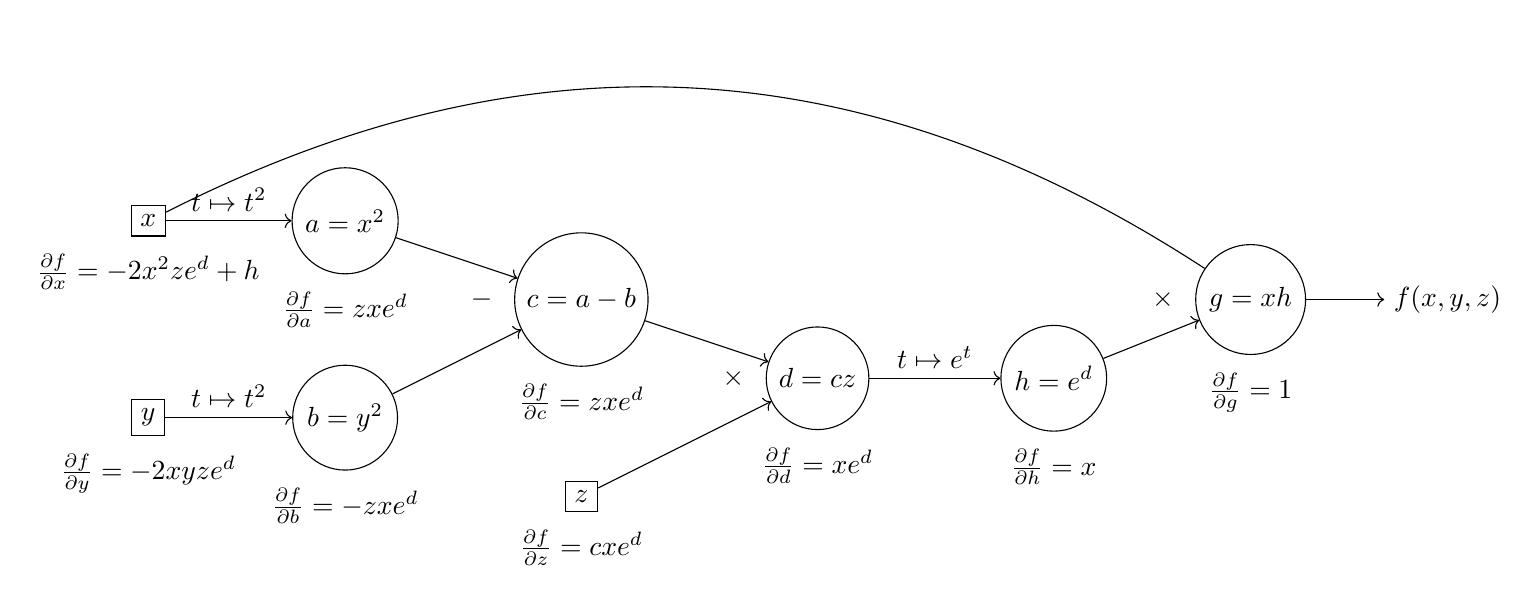
\begin{tikzpicture}
	
	% Nodes
    \node[draw, rectangle] (x) at (0.5, 0) {$x$};
    	\node [below=0.1 of x] {$\frac{\partial f}{\partial x} = -2x^2ze^d + h $};
    \node[draw, rectangle] (y) at (0.5, -2.5) {$y$};
        \node [below=0.1 of y] {$\frac{\partial f}{\partial y} = -2xyze^d$};
    \node[draw, rectangle] (z) at (6, -3.5) {$z$};
        \node [below=0.1 of z] {$\frac{\partial f}{\partial z} = cxe^d$};

    \node[draw, circle] (a) at (3, 0) {$a=x^2$};
        \node [below=0.1 of a] {$\frac{\partial f}{\partial a} = zxe^d$};
    \node[draw, circle] (b) at (3, -2.5) {$b=y^2$};
        \node [below=0.1 of b] {$\frac{\partial f}{\partial b} = -zxe^d$};
    \node[draw, circle] (c) at (6, -1) {$c=a - b$};
        \node [below=0.1 of c] {$\frac{\partial f}{\partial c} = zxe^d$};
    \node (minsymb) [left=0.15 of c] {$-$};
    \node[draw, circle] (prod) at (9, -2) {$d=cz$};
        \node [below=0.1 of prod] {$\frac{\partial f}{\partial d} = xe^d$};
    \node (multsymb) [left=0.15 of prod] {$\times$};
    \node[draw, circle] (exp) at (12, -2) {$h=e^d$};
        \node [below=0.1 of exp] {$\frac{\partial f}{\partial h} = x$};
    \node[draw,circle] (prodfin) at (14.5,-1) {$g=xh$};
    	\node [below=0.1 of prodfin] {$\frac{\partial f}{\partial g} = 1$};
    \node [left=0.15 of prodfin] {$\times$};
    \node (out) at (17,-1) {$f(x,y,z)$};
    
    % Arrows
    \draw[->] (x) -- node[midway,above] {$t \mapsto t^2$} (a);
    \draw[->] (y) -- node[midway,above] {$t \mapsto t^2$} (b);
    \draw[->] (a) -- (c);
    \draw[->] (b) -- (c);
    \draw[->] (c) -- (prod);
    \draw[->] (z) -- (prod);
    \draw[->] (prod) -- node[midway,above] {$t \mapsto e^t$} (exp);
    \draw[->] (exp) -- (prodfin);
    \path[bend left=30] (x) edge (prodfin);
    \draw[->] (prodfin) -- (out);	
	
	\end{tikzpicture}
	
\label{fig:backward_pass_ex}
\caption{Exemple de \textit{backward pass}.}
\end{figure}

Les graphes de calcul tels que représentés précédemment permettent de simuler une exécution du réseau de neurones ou de la fonction considérée. Cependant, leur intérêt ne se limite pas à cela puisqu'ils permettent aussi de calculer efficacement le gradient de la fonction considérée en remontant le graphe, c'est la \textit{backward pass}.

L'idée repose sur la règle de la chaine : 
	$$ \frac{\partial f}{\partial x} = \underset{y \text{ child of }x}{\sum} \frac{\partial y}{\partial x} \frac{\partial f}{\partial y} $$
	
	Formellement, on voit d'abord $f$ comme une fonction de $g$ (la fonction identité) et on a donc $\frac{\partial f(g)}{\partial g} = 1$. Puis on voit $g$ comme une fonction de $x$ et $e$ et on a $\frac{\partial f(g(x,e))}{\partial e}=x$, puis on voit $e$ comme une fonction de $d$ et ainsi de suite jusqu'à obtenir $\frac{\partial f}{\partial x}$, $\frac{\partial f}{\partial y}$ et $\frac{\partial f}{\partial z}$ qui sont les trois coordonnées du gradient de $f$.\\
	
	Le résultat de ces opérations sur le graphe de calcul est montré en figure \ref{fig:backward_pass_ex}.

\section{Provenance}

Nous souhaitons abstraire les méthodes précédentes à travers une strucuture algébrique adaptée, de façon analogue à la provenance par semi-anneaux dans les bases de données introduite dans [Green et al.].

	\subsection{Généralisation par les semi-anneaux}

	L'idée la plus directe consiste à remplacer

	\subsection{Généralisation}

	Du point de vue de cette provenance fine, on distingue trois grandes catégries d'objets. La première est constituée des éléments $x_1$, $x_2$ de l'input et des biais $b$, la deuxième est constituée des coefficients des matrices $a_{i,j}$ et la troisième est constituée de fonctions $f$. Nous appelons $E$ le premier ensemble, $A$ le deuxième et $F$ le troisième.
	
	Afin d'abstraire ce fonctionnement, il convient de trouver des structures adaptées pour ces trois catégories. Pour cela nous commençons par quelques observations :
	
	\begin{itemize}
	
		\item Les coefficients $a_{i,j}$ agissent sur les coefficients $x_{i}$, par une application 
		$\left\lbrace \begin{array}{c c c}
		 A \times E & \to & E \\
		 (a,x) & \mapsto & ax
\end{array}
\right.$
		
		\item L'ensemble $E$ est muni d'une opération $+$.
	
	\end{itemize}

\end{document}